% !TEX root = thesis.tex
\graphicspath{ {./figures/} }

%%%%%%%%%%%%%%%%%%%%
\chapter{Evaluation}
%%%%%%%%%%%%%%%%%%%%

%%%%%
\TODO{put this somewhere in this section, its about using inverse dict of dict instead of normal dict of dict}

Despite all algorithms taking in put in inverse dict-of-dicts format, there may still be preprocessing necessary. While the iterative solver can use the inverse dict-of-dicts directly, using it as a lookup table as it spreads power around the graph, the system of linear equations need to be constructed from the dict-of-dicts input. Including such set-up time in benchmarks may be misleading, as this time is not spent on actually resolving delegations, thus only the time spent actually resolving the delegations is used, and any set-up time is ignored. Nevertheless, in practice, the set-up time can be a relevant factor—depending on the use case and data format—when choosing between different approaches or implementations. The set-up procedures required for each implementation are described in more detail in the sections below.

\TODO{Fix and improve all graphs, especially title and labels...}

The three algorithms will be evaluated based on their runtime and scalability. The evaluation will first cover synthetically generated graphs including randomly generated small and big graphs as well as corner cases, then graphs generated based on social behaviors, so-called social graphs, and finally graphs based on real-world datasets.

\section{Method}

\subsection{Generating Random Delegation Graphs}

For the first section, we built an algorithm, that builds a graph with n nodes, and then adds between zero and three delegations per node to random other nodes, ensuring that there are no delegation cycles without a sink. A better explanation of how these graphs are artificially constructed can be found in the Annex. \TODO{Create this annex} We acknowledge, that these assumptions may not be representative of real delegation graphs, where, as studies have shown, delegates tend to not delegate randomly, but to a subset of experts, such as TV personalities, thus centering power to one or few people. This approach also overlooks potential tendencies of voters, such as delegating to individuals they perceive as more competent or confident than them, or the tendency of power to concentrate among a few, very popular so-called "super-voters" \cite{klingVotingBehaviourPower2015}. These concerns are addressed in section XX, when we benchmark delegation graphs that are based on social graphs. 


\subsection{Preprocessing}

In order to be able to benchmark algorithms that resolve delegations, the input graphs need to be well-formed delegation graphs. In section XX and YY, we use graphs which are not well-formed delegation graphs out-of-the-box. This subsection details the process of how any arbitrary graphs, including undirected and unweighted graphs, can be turned into well-formed delegation graphs. An overview of this process is shown in \cref{fig:cleaning_process}.

\begin{figure}[h]
    \centering
    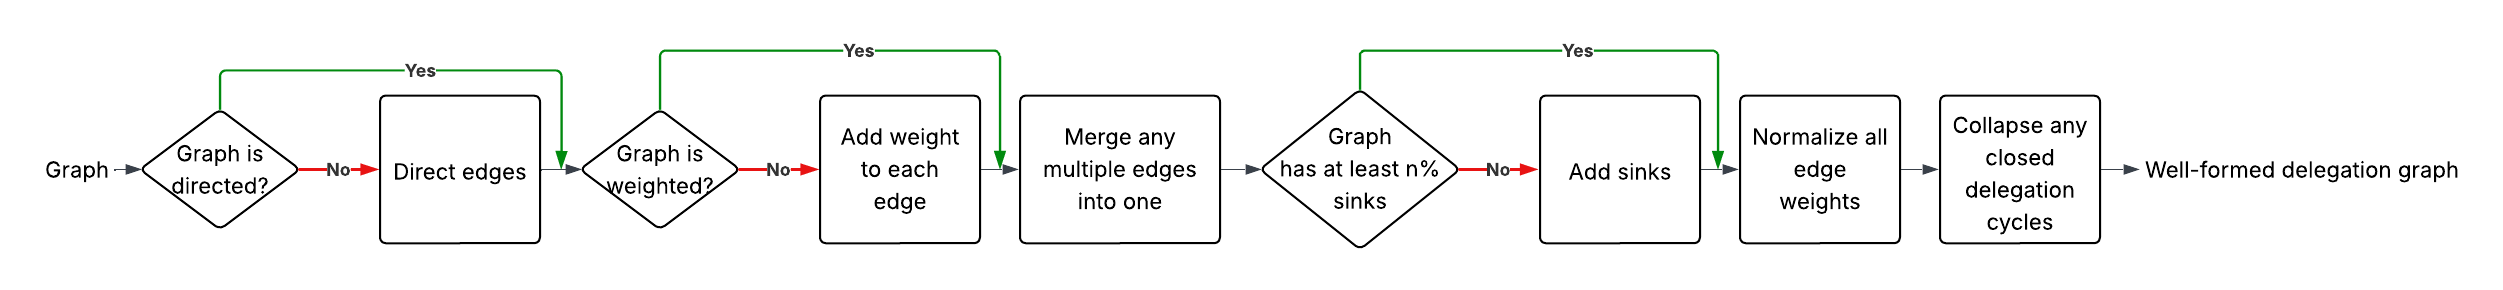
\includegraphics[width=\textwidth]{Thesis Evaluation Methodology Process.png}
    \caption{Process to clean any graph into a delegation graph.}
    \label{fig:cleaning_process}
\end{figure}

If the graph is undirected, is it given a direction. This is done arbitrarily, with the algorithm interpreting undirected edges in the shape $(u, v)$ as directed edges from u to v. If the algorithm fails to find a weight for an edge, it will also assign it a weight of one. Next, any multiple edges, so parallel edges going from the same node to the same node are merged, with any weights being added together. If less than $n\%$ of the graph's nodes are sinks, the algorithm randomly removes all outgoing delegations of delegators, turning them into sinks. By default this n value is 20, however depending on the use case it can be increased or decreased. After this, the algorithm searched for any closed delegation cycles, and collapses all it finds into a single sink node. Specifically, the algorithm searched for strongly connected components (STCCs) in the graph, so components of the graph where each node can reach each other node, and checks if it it is a closed delegation cycle, by checking if any of the nodes within this STCC to a node outside of the STCC. An exception to this are sinks who have no delegators, these are technically STCCs with no outgoing edges, however they are not closed delegation cycles. All closed delegation cycles are collapsed into a "lost" node, which means that any delegations to the cycle get re-directed to a specially created node. The resulting graph from this operation is a well-formed delegation graph, since all power that flows into closed delegation cycles now flows into a sink, so the graph is free of closed delegation cycles.

\subsection{Measurement}

Despite all algorithm's taking in put in inverse dict-of-dicts format, there may still be preprocessing necessary. While the iterative solver can use the inverse dict-of-dicts directly, using it as a lookup table as it spreads power around the graph, the other solver require the system of linear equations in specific formats, which need to be set up from the inverse dict-of-dicts input. Including such set-up time in benchmarks may be misleading, as this time is not spent on actually resolving delegations, thus we separated the set-up and resolving, and in the benchmarks only the time spent actually resolving the delegations is used; any set-up time is ignored. Nevertheless, in practice, the set-up time can be a relevant factor—depending on the use case and data format—when choosing between different approaches or implementations. The set-up procedures required for each implementation are described in more detail in the sections below.

To minimize the impact of background noise and measurement fluctuations on the benchmarks, algorithms with very short runtimes were executed multiple times, and the average runtime was recorded. The recorded runtimes always indicate just the runtime for the algorithms to resolve the delegations, times for set-up, such as the time for building the linear program, were not included. 

% cont here, merge the old benchmark stuff into these new sections, and add the new data

\section{Synthetic Graphs}

\subsection{Small Graphs}
\label{subsec:small_graphs}

\begin{figure}[h]
    \centering
    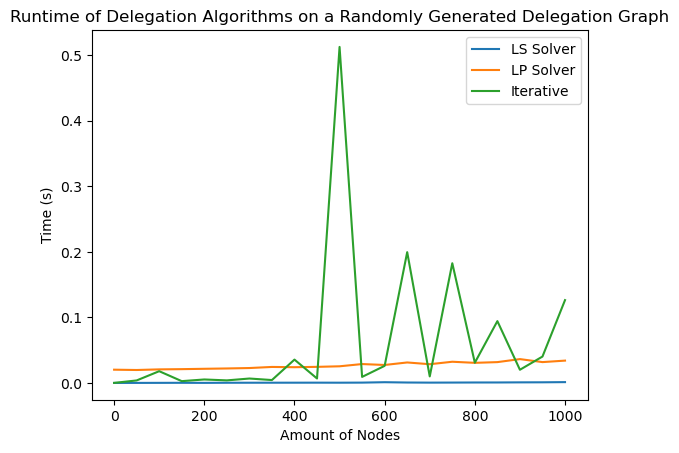
\includegraphics[width=0.4\textwidth]{0-1000_random}
    \caption{Runtime of delegation algorithms on a randomly generated delegation graph.}
    \label{fig:random-small}
\end{figure}

In order to explore the three algorithm's behavior on small graphs, we used the graph generator to generate graphs with zero to 1000 nodes. \Cref{fig:random-small} shows the results of this benchmark.

We can see, that the LS Implementation, optimized for sparse matrices, outperforms the other two algorithms. Its growth in runtime is so small, that the line looks to be staying flat on the x-axis. However, with a graph of 1000 nodes, its runtime is about 0.01 seconds. Both the LS and LP implementation display a rather steady, yet growing runtime. The LP solver seems to have some overhead, since even when the graph has zero nodes, it has a runtime of about 0.02 seconds.

Furthermore, we can interestingly observe large spikes in the runtime of the iterative approach. Exploring this more closely, we find that the graph with 11 nodes takes the iterative algorithm a lot more time than the graph with 10 or 12 nodes, as shown in \cref{fig:random-tiny}. At 10 nodes, the runtime of the iterative algorithm is just about 0.004 seconds, at 12 nodes it is 0.001 seconds, so even slightly faster than the slightly smaller graph, but when the graph has 11 nodes, the runtime skyrockets to about 0.056 seconds.

\begin{figure}[h]
    \centering
    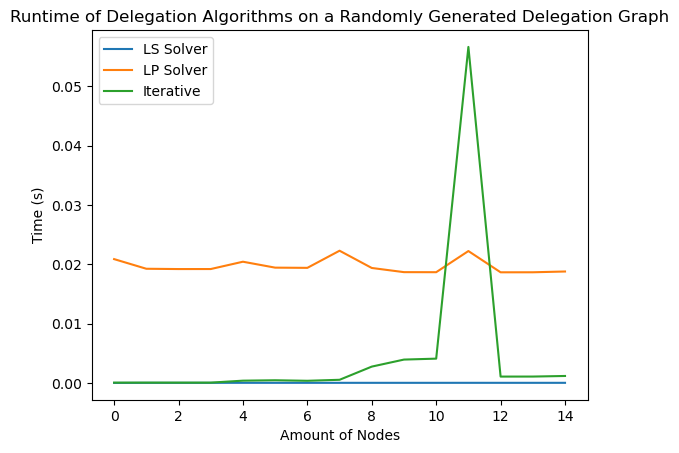
\includegraphics[width=0.4\textwidth]{0-15_random}
    \caption{Runtime of delegation algorithms on a randomly generated delegation graph.}
    \label{fig:random-tiny}
\end{figure}

A possible explanation for this spike may be, that when the graph has 10 and 12 nodes, it iterates only 758 and 170 times respectively, before cutting off, while when it has 11 nodes it iterates 8735 times before cutting off. \Cref{fig:random-11and12} shows the two graphs with 11 and 12 nodes.

\begin{figure}[h]
    \centering
    \begin{subfigure}[t]{0.45\textwidth}
        \centering
        \fbox{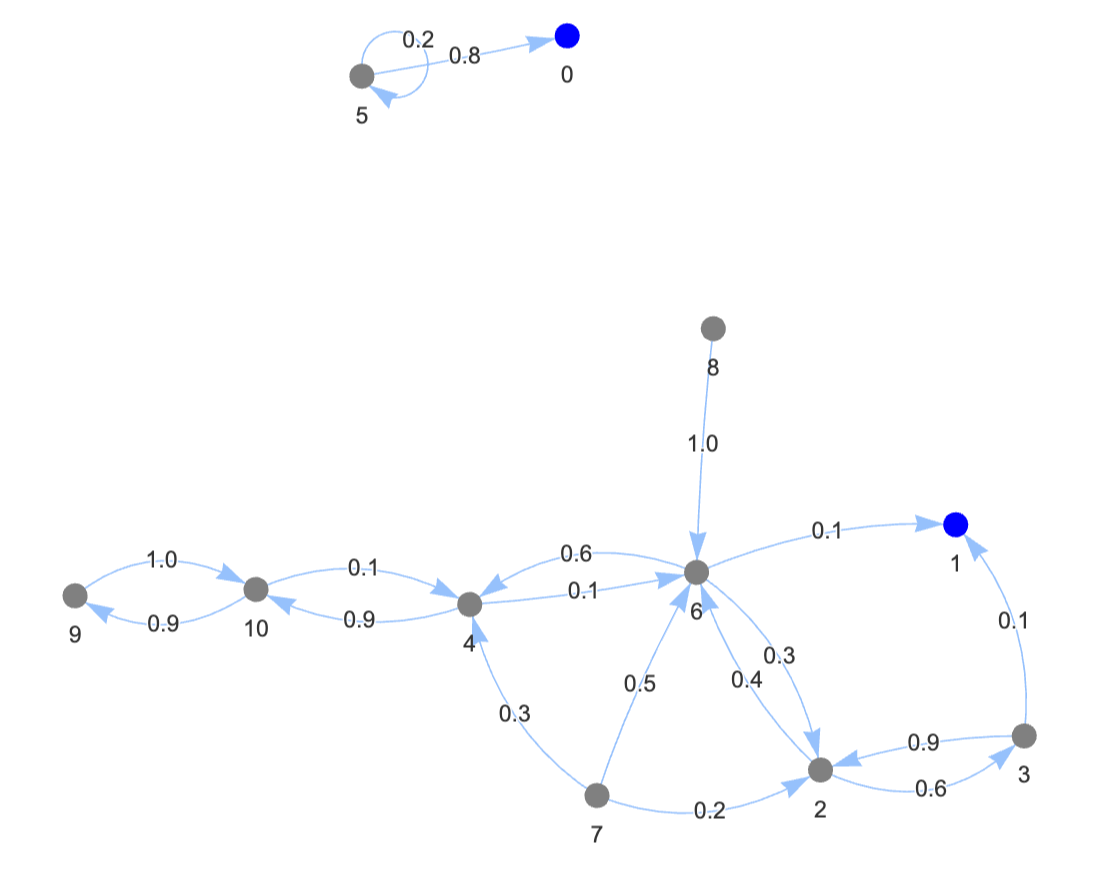
\includegraphics[width=\textwidth]{11_random}}
        \caption{11 nodes}
        \label{subfig:random-11and12-11}
    \end{subfigure}
    \hfill
    \begin{subfigure}[t]{0.45\textwidth}
        \centering
        \fbox{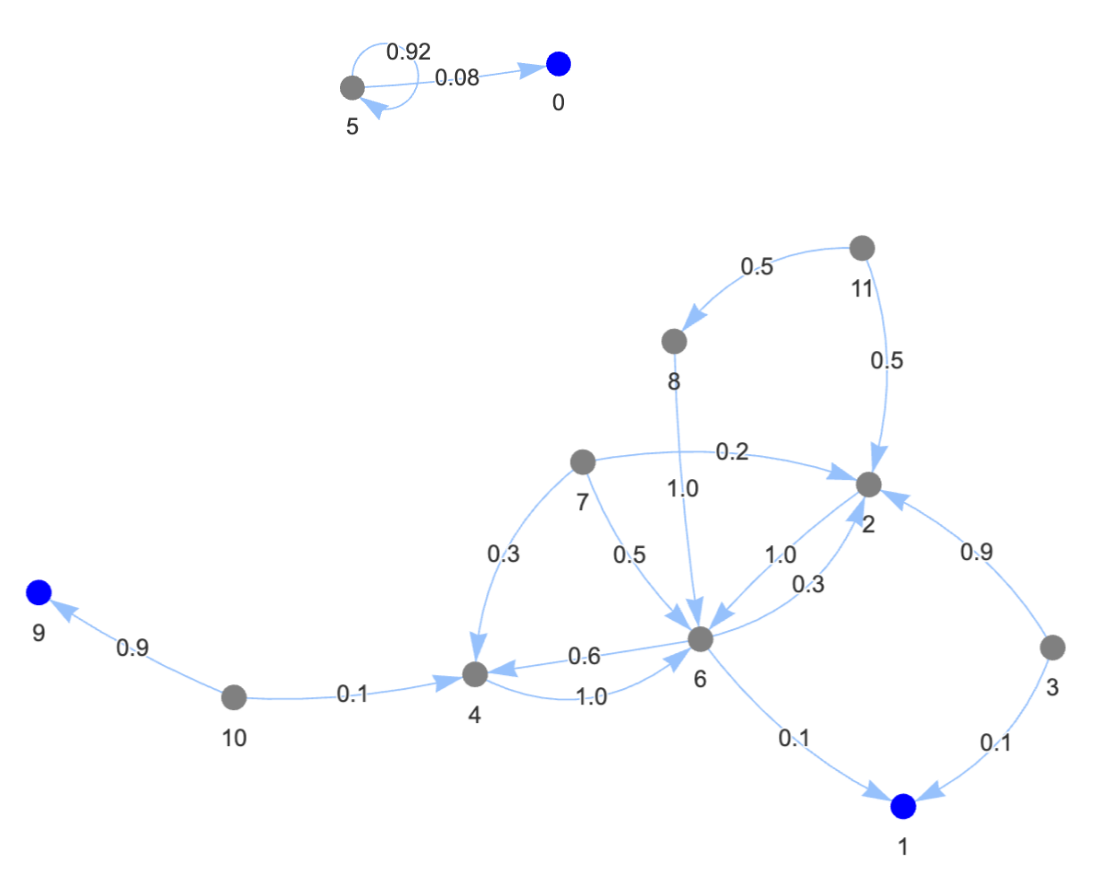
\includegraphics[width=\textwidth]{12_random}}
        \caption{12 nodes}
    \end{subfigure}
    \caption{Delegation graphs with 11 and 12 nodes (Blue nodes are sinks)}
    \label{fig:random-11and12}
\end{figure}

Inspecting the graphs reveals a possible explanation for this behavior. When the graph has 12 nodes, node \texttt{9} is a sink, while in the graph with 11 node it delegates its power back to node \texttt{10}. In the latter case, power going out of node \texttt{9} needs to pass to node \texttt{10}, \texttt{4} and \texttt{6} before reaching a sink. While passing through node \texttt{4}, we can see that 90\% of the power is delegated back into the cycle between nodes \texttt{4}, \texttt{10} and \texttt{9}. The algorithm will iterate power through this loop, until enough has been drained out for the \texttt{total\_change} to fall below the cutoff. 

This is an important shortcoming of the iterative algorithm. Power can easily get trapped within permissible delegation cycles that only have a small drain allowing the power to escape from the cycle. Each iteration, if a great proportion of the nodes with draining edges' power is sent back into a cycle, the algorithm needs to continuously iterate until the power is back at the drain nodes, however depending on the cycle this may happen very inefficiently. This phenomenon will be tested more in \cref{subsec:cycles_draining}

\subsection{Large Graphs}

Delegation graphs may grow arbitrarily large. National elections for example can contains up to hundreds of millions of participants. This section explores how the algorithms perform when having to resolve graphs with a lot of nodes. Again, the graphs will be randomly generated, such that each nodes has between 0 and 3 delegates. 

\begin{figure}[h]
    \centering
    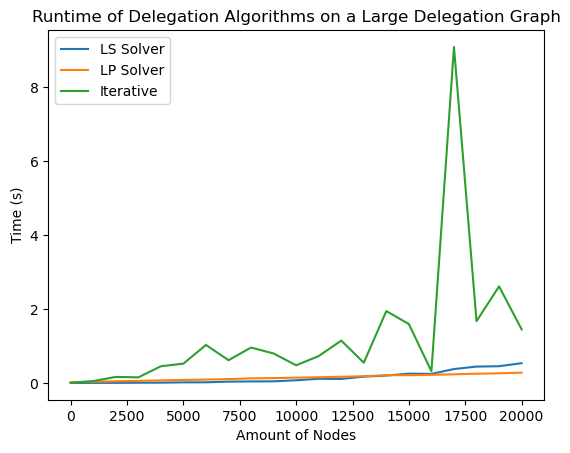
\includegraphics[width=0.4\textwidth]{0-20000_random}
    \caption{Runtime of delegation algorithms on a randomly generated delegation graph.}
    \label{fig:random-large}
\end{figure}

In \cref{fig:random-large} we can see, that it is difficult to determine a pattern in the runtime for the iterative algorithm. Depending on the underlying delegation graph, the runtime can grow unpredictably large. What is evident from the runtime graph however, is that in as the graphs get larger its runtime never subceeds the runtimes of the other two algorithms, while it is worth mentioning that for some graphs, the iterative algorithm's runtime is not a lot longer than that of the other two algorithms. It is difficult to make any statement about the runtime class of the iterative algorithm based just on the number of nodes in the graph, since, depending on the structure of the graph and the cutoff value the runtime can get arbitrarily high. The comparatively high runtime of the iterative algorithm overshadows the runtimes of the other two, so in order to better discuss and analyze their performance, \cref{fig:random-large-no-iterative} shows the same graph as in \cref{fig:random-large}, without the runtimes for the iterative algorithm.

\begin{figure}[h]
    \centering
    \begin{subfigure}[t]{0.45\textwidth}
        \centering
        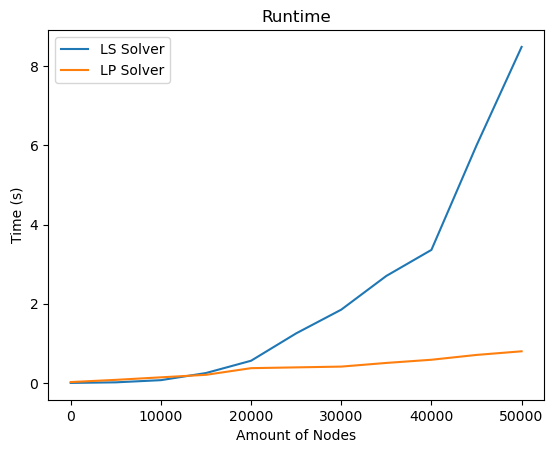
\includegraphics[width=\textwidth]{0-50000_random_no_iterative}
        \caption{Linear scale}
         \label{subfig:random-large-no-iterative-linear}
    \end{subfigure}
    \hfill
    \begin{subfigure}[t]{0.45\textwidth}
        \centering
        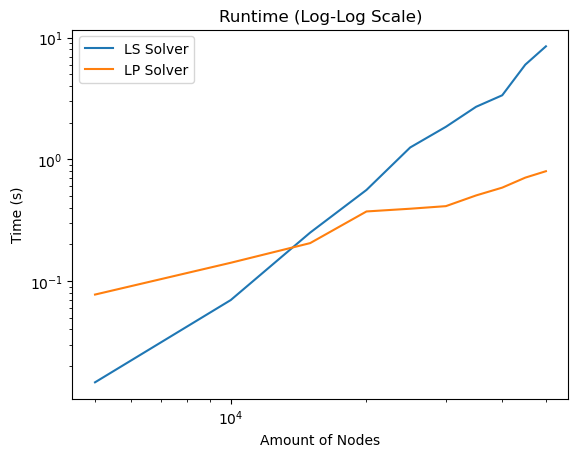
\includegraphics[width=\textwidth]{0-50000_random_no_iterative_loglog}
        \caption{Loglog scale}
         \label{subfig:random-large-no-iterative-loglog}
    \end{subfigure}
    \caption{Runtime of delegation algorithms on a randomly generated delegation graph.}
    \label{fig:random-large-no-iterative}
\end{figure}

\begin{figure}[h]
    \centering
    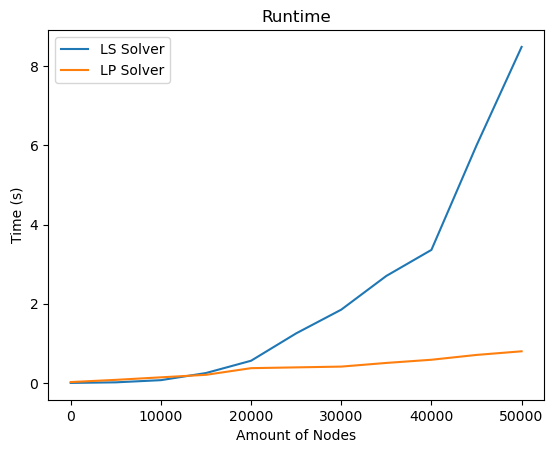
\includegraphics[width=0.4\textwidth]{0-50000_random_no_iterative}
    \caption{Runtime of delegation algorithms on a randomly generated delegation graph.}
    \label{fig:random-large-no-iterative}
\end{figure}

\Cref{subfig:random-large-no-iterative-linear} shows, that as the delegation graph grows, the LP solver's runtime grows more slowly than the LS Solver's. For resolving smaller graphs, the LS solver outperforms the LP solver, with a runtime of almost zero for empty or very small graphs, while the LP solver has a clearly non-zero runtime even for very small graphs. However, at around 12 000 nodes, this changes, as the LP solver's runtime's slower growth catches up with that of the LS solver. 

The type of growth, so the runtime class, is not immediately clear from the graphs, although the LP solver's growth seems to be more linear than that of the LS solver. Looking at the same results on a loglog graph reveals, that the LS solvers runtime may follow a power law.

Fitting the data into different kinds of curves reveals, that the LP implementations runtime likely has linear growth, while the LS solver grows following a power distribution, such that it is in the runtime class of $O(n^{2.778})$.

\TODO{Put the runtime results and/or the code and the regression results into the annex, or into the text...}

\subsection{Dense Graphs}

While we expect most delegators in any delegation graph to only delegate to a handful of people, a well formed delegation graph can have any number of delegates per delegator. Thus, it is also interesting to compare how the three algorithms compare when resolving more dense graphs. In this section, we test the three implementations on NetworkX's $G_{n,p}$ graph generator \texttt{gnp\_random\_graph}, which returns a directed graph with $n$ nodes, where each node connected to each other node with probability $p$, which is set to $0.5$ for the remainder of this section \cite{hagbergExploringNetworkStructure2008}. These graphs are not well-formed delegation graphs out-of-the box, thus we adapt them by removing outgoing edges of nodes, turning them into sinks, until 10\% of the nodes are sinks. Then, each delegators vote is equally distributed to all of its outgoing edges, such that the edge weights add up to 1. Finally, any closed delegation cycles are removed by removing a random edge in the cycle (and re-normalizing the edge weights). 

\begin{figure}[h]
    \centering
    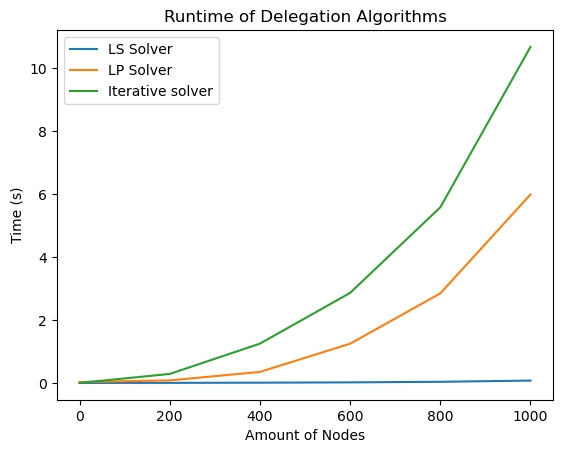
\includegraphics[width=0.4\textwidth]{0-1000_dense}
    \caption{Runtime of delegation algorithms on a randomly generated delegation graph.}
    \label{fig:dense-small}
\end{figure}

\Cref{fig:dense-small} shows the runtime of these three algorithms. The runtime of the iterative algorithm lacks the spikes found when resolving sparse graphs. This is likely due to the nature of the graphs we create. Every delegator is connected to half of all other nodes ($p = 0.5$), and of these $10\%$ are sinks, thus power drains quickly into sinks, and situations where power iterates a long time without seeing a sink are less frequent. Regardless, the iterative algorithm exhibits the worst runtime of the three. 

\begin{figure}[h]
    \centering
    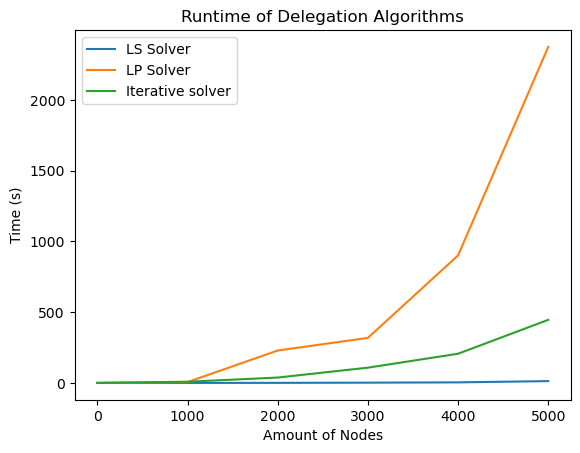
\includegraphics[width=0.4\textwidth]{0-5000_dense}
    \caption{Runtime of delegation algorithms on a randomly generated delegation graph.}
    \label{fig:dense-large}
\end{figure}

Testing the three algorithms on larger dense graphs, reveals surprisingly, that the LP solver's runtime is considerably worse than that of both the iterative and LS solver. A dense graph with 5,000 nodes, and thus about 125,000 delegations, takes the LS solver only about 12 seconds, the iterative solver 445 seconds, and the LP solver almost 2,400 seconds. Even though the LS solver is optimized for sparse matrices, it outperforms the other two implementations on dense graphs.

\subsection{Cycles Which Retain a Lot of their Power}

\label{subsec:cycles_draining}

\begin{figure}[h]
	\centering
	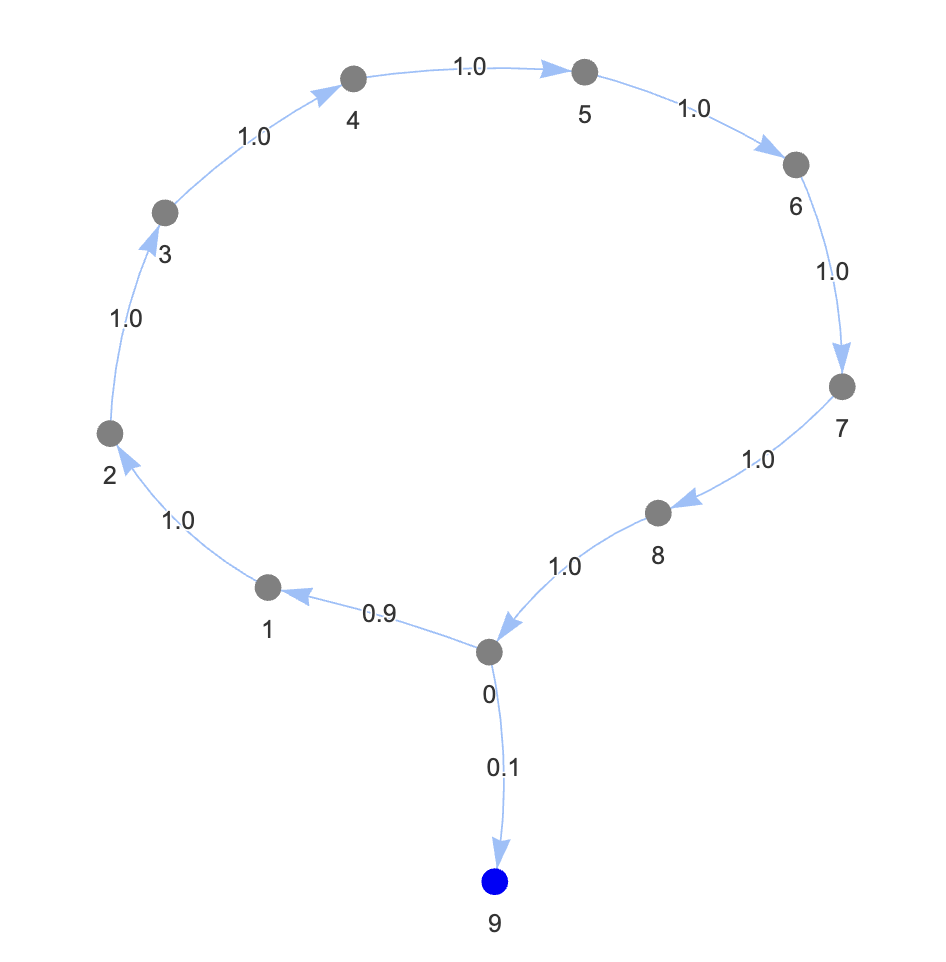
\includegraphics[width=0.4\textwidth]{big_cycle_example}
	\caption{An example of the cycles used for the benchmarks. The blue node is the sink}
	\label{fig:big_cycle_example}
\end{figure}

To further explore one of the iterative algorithm's shortcomings, this section will explore and compare runtime behavior for delegation cycles which are not closed, but contain only few, weak edges for power to drain, thus forcing power to iterate around in the cycle before it reaches a sink. Specifically, we construct graphs with delegates all delegating power to the next node in the cycle. One node in the cycle contains an edge with weight 0.1 to a sink, while the other 0.9 of its power go to the first node in the cycle. \Cref{fig:big_cycle_example} contains an exemplary image of such a graph with 10 nodes. 

\begin{figure}[h]
    \centering
    \begin{subfigure}[t]{0.45\textwidth}
    	\centering
    	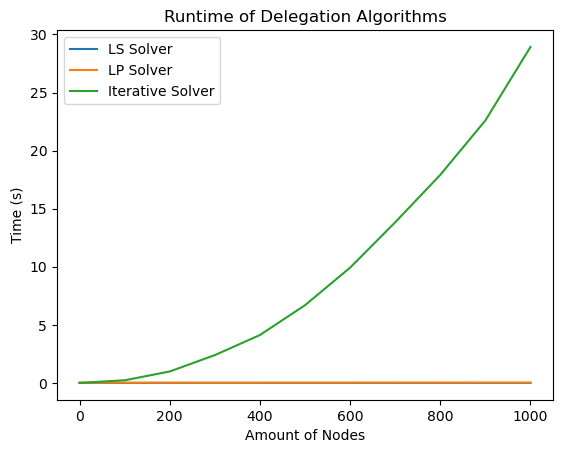
\includegraphics[width=\textwidth]{0-1000_cycle}
    	\caption{Linear scale}
    	\label{subfig:cycle-small-linear}
    \end{subfigure}
    \hfill
    \begin{subfigure}[t]{0.45\textwidth}
        \centering
        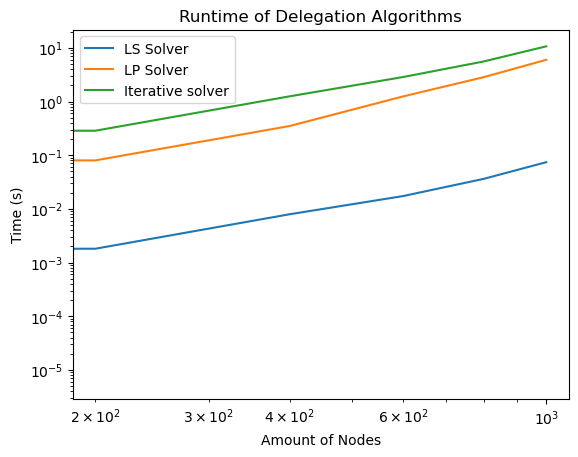
\includegraphics[width=\textwidth]{0-1000_dense_loglog}
        \caption{Loglog scale}
         \label{subfig:cycle-small-loglog}
    \end{subfigure}
    \caption{Runtime of delegation algorithms on a randomly generated delegation graph.}
    \label{fig:cycle_small}
\end{figure}

The runtimes in \cref{subfig:cycle-small-linear} show, that as expected, the iterative algorithm struggles considerably with the resolution of these graphs, while the other two algorithms exhibit behavior similar to that on randomly generated sparse delegation graphs. The growth of the runtimes seems to be polynomial, with the iterative algorithm belonging to the runtime class $O(n^{2.12})$. Being able to resolve these kinds of loops is one of the greatest strength of the two approaches, which don't simulate power as flow through the graph. By directly solving the system of linear equations, they are a lot more well equipped to deal with this specific corner case.  

\begin{figure}[t]
	\centering
    	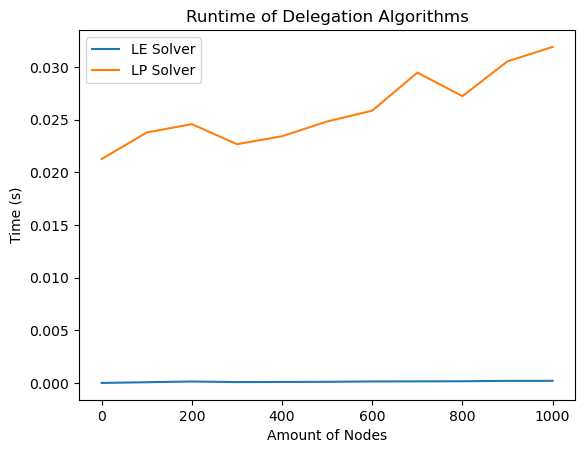
\includegraphics[width=0.4\textwidth]{0-1000_cycle_no_iterative}
    	\caption{Runtime of delegation algorithms on a randomly generated delegation graph.}
	\label{fig:cycle-small-no-iterative-linear}
\end{figure}

As seen in \cref{fig:cycle-small-no-iterative-linear}, which shows the same graph as in \cref{subfig:cycle-small-linear} without the iterative algorithm's runtime, the runtime of the LS and LP Solvers grows similarly to when resolving randomly generated (sparse) delegation graphs, such as the ones found in \cref{subsec:small_graphs}.

Such a cycle as the one we deliberately constructed is not the only situation in which the iterative algorithm will struggle. As long as power is not efficiently funneled toward a sink, the iterative algorithm will have to spend more time moving the power around until enough has drained into a sink for \texttt{total\_change} to fall below the cutoff value. A further example of such behavior is the cycle that caused runtime to spike in \cref{subfig:random-11and12-11}. An artificial example of this situation is shown below in Figure XX. \TODO{Create this graph}

\section{Social Graphs}

Social graphs provide an excellent way to \TODO{Finish this sentence}... We will use them to create sample delegation graphs based on social behaviors, which can predict ways humans may delegate if given the chance to delegate fractionally. These graphs are still only based on models, however since they are artificial, we can scale them and explore how the algorithms scale.

\TODO{For each social graph, include a sentence or two on why its good}

\subsection{Small World Graphs}

\TODO{Introduce those woganotiz stroff Small World graphs and the way I generated them (with prepare\_graph 20\% sinks, etc.)}

\begin{figure}[h]
    \centering
    \begin{subfigure}[t]{0.45\textwidth}
        \centering
        \fbox{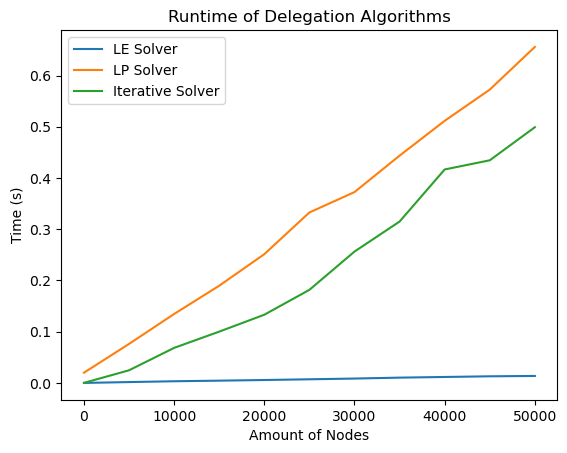
\includegraphics[width=\textwidth]{0-50000_small_world}}
        \caption{Linear scale}
        \label{subfig:small_world_graph_linl}
    \end{subfigure}
    \hfill
    \begin{subfigure}[t]{0.45\textwidth}
        \centering
        \fbox{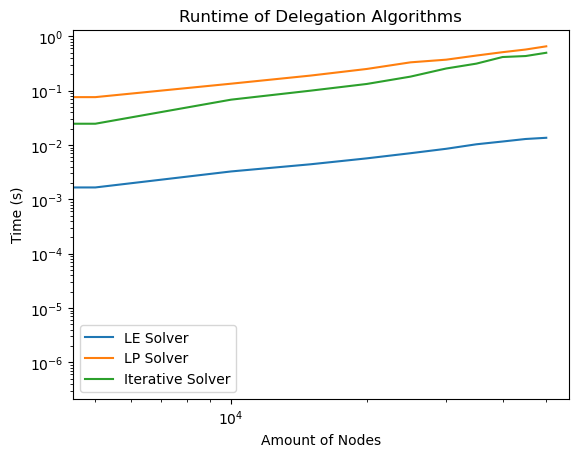
\includegraphics[width=\textwidth]{0-50000_small_world_loglog}}
        \caption{Loglog scale}
        \label{subfig:small_world_graph_loglog}
    \end{subfigure}
    \caption{Runtime of delegation algorithms on a randomly generated delegation graph.}
    \label{fig:small_world_graph}
\end{figure}

Fig XX shows the results of the benchmarks on these graphs. 

\subsection{R-Mat Graphs}

\TODO{Remove the comments under this line in the .tex file}
%\subsection{Stochastic Block Model Graph}
%
%\TODO{This whole section is an incomplete mess, but verify it with Prof. Ford before putting more effort into it.}
%
%Stochastic block model graphs partition nodes into groups, and place edges between nodes of each group according to specified probabilities. This allows us to model a hierarchy of voters with different levels of confidence, where voters with a higher confidence are more likely to vote themselves, and voter with a lower confidence have a tendency to delegate to voters with a higher confidence. Revel et al. show this phenomenon can be observed in practice. \cite{revel2022liquid} 
%
%Specifically, the nodes in the graphs for this section are partitioned into three groups. 60\% of nodes are voters with low confidence,  30\% of voters have medium confidence, and 10\% of voters have high confidence. NetworkX's \texttt{stochastic\_block\_model} graph generator takes as input the sizes of each group, as well as a matrix specifying the density of edges between two groups that should be added. A density of $p_{X, Y} = 1$ between groups X and Y would mean that every possible edge from all nodes in group X to all nodes in group Y is added to the graph, while a density of $p_{X, Y} = 0.5$ suggests that only half this amount is added. Each density is applied to a set of edges of size $|X||Y|$. With a growing amount of edges in the graph, both $|X|$ and $|Y|$ grow, thus $p_{X, Y} |X||Y|$ is a constant multiplied by two linearly growing terms, and thus exhibits squared growth. In other words, with the density set like this, the amount of outdoing edges per node increases as the total amount of nodes increases. This is not desirable, as it would suggest that each voter's tendency to delegate depends on the total size of the delegation graph. However, realistically, each voter's social circle has a constant size, regardless of how many voter participate in total. We thus add a dividing factor of $\sqrt{|X||Y|}$ to each $p_{X, Y}$ term in order to cancel out this effect. 
%
%Each delegation graph $G = (V, E)$ with $n$ nodes is thus partitioned into three subsets, $L \dot\bigcup M \dot\bigcup H = V$ (low confidence, medium confidence and high confidence), of sizes 
%
%\begin{align*}
%|L| &= 0.6|V|, \\
%|M| &= 0.3|V|, \\
%|H| &= 0.1|V|
%\end{align*}
%
%To implement the tendency to trust more competent individuals and thus delegate to them more likely, we set up the following densities.
%
%Let $p_{\mathrm{up}} = 0.8$ denote the probability mass for delegations to higher-confidence groups, $p_{\mathrm{same}} = 0.2$ the probability mass for delegations within the same group, and $p_{\mathrm{down}} = 0.05$ the probability mass for delegations to lower-confidence groups. These probabilities are scaled according to the group sizes in order to ensure that the total expected number of outgoing delegations per voter remains constant as the graph grows.
%
%The resulting density matrix $P$ is defined as follows, where rows correspond to the delegator's group and columns correspond to the recipient's group:
%
%\[
%matrix with probabilities
%\]
%
%This matrix reflects the intended behavior: 
%\begin{itemize}
%    \item Voters in the low-confidence group $L$ mostly delegate upwards to medium- and high-confidence voters, with a moderate chance to delegate within their group.
%    \item Voters in the medium-confidence group $M$ predominantly delegate within their group or upwards to high-confidence voters, while rarely delegating downwards.
%    \item Voters in the high-confidence group $H$ delegate mostly within their group and rarely downwards, modeling their higher self-confidence and status in the network.
%\end{itemize}
%
%\TODO{Somewhere mention how fidly this is, since if you made delegations to lower or mid too high you get loads of cycyles, and theyre quite bad, since in this implementation they lead to closed delegation cycles quickly}
%In the implementations for this section, it is assumed that more competent voters vote to less competent voters 10\% of the time, to voters with the same confidence 40\% of the time, and to voters with higher confidence 
%
%
%
%\begin{figure}[h]
%    \centering
%    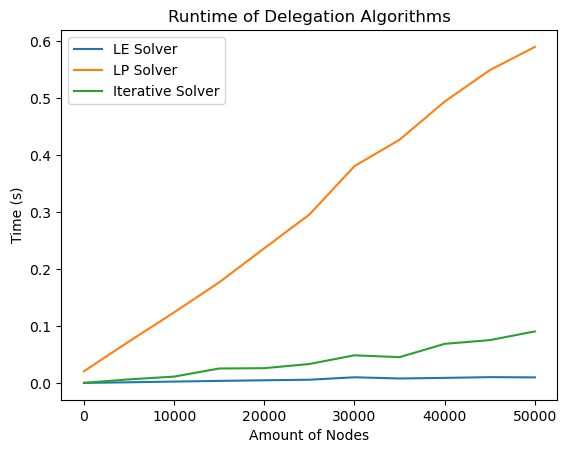
\includegraphics[width=0.4\textwidth]{0-50000_sbm}
%    \caption{Runtime of delegation algorithms on stochastic block model graphs.}
%    \label{fig:sbm}
%\end{figure}
%
%Fix XX shows the runtimes of the three implementations as the amount of nodes in these graphs increases. Similarly to the small world graphs, the linear programming solver exhibits the worst runtime, followed by the iterative implementation, and then the linear system solver implementations. However, it seems, that the iterative implementation's runtime grows less quickly. In the previous section, every node had about three outgoing edges, while in this implementation only about every other node has an outdoing edge, as shown in fig XX. This suggests, that the distance between delegators and their nearest sink is likely very short, since every other node is a sink. \TODO{Add to this explanation, that the way the graphs are generated also means that nodes reach sinks quickly}. As a result, the graphs are (largely?) free of cycles, which the iterative algorithm can handle especially well, since it does not have to iterate power through cycles. 
%
%\begin{figure}[h]
%    \centering
%    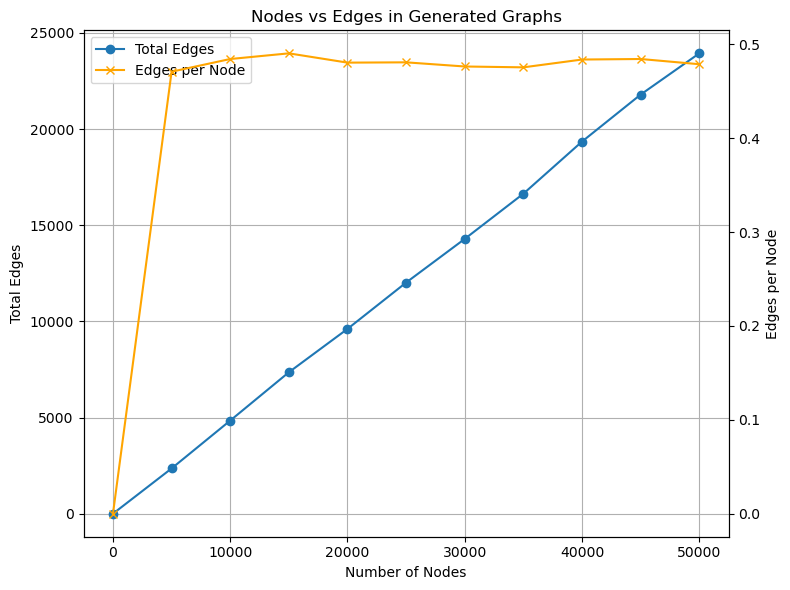
\includegraphics[width=0.4\textwidth]{sbm_edge_growth}
%    \caption{Growth of edges as the amount of nodes increase in the delegation graphs based on stochastic block model graphs.}
%    \label{fig:sbm_edge_growth}
%\end{figure}
%
%
%\subsection{Supervoter}
%
%\begin{figure}[h]
%    \centering
%    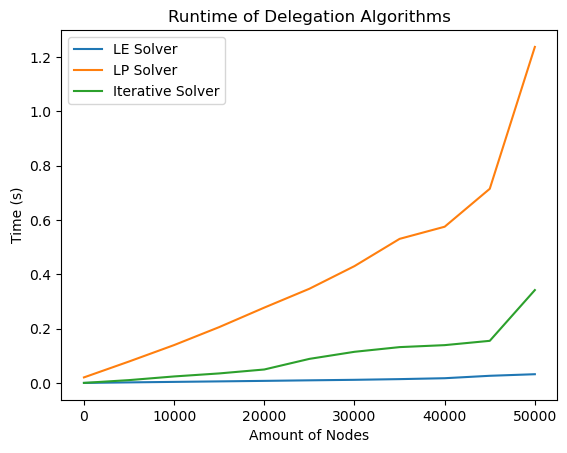
\includegraphics[width=0.4\textwidth]{0-50000_supervoter}
%    \caption{Runtime of delegation algorithms on supervoter graphs.}
%    \label{fig:supervoter}
%\end{figure}

\section{Real-World Datasets}

This section evaluates the three algorithms on some real-world datasets. While liquid democracy without fractional delegation has been implemented and tested in studies \TODO{Cite}, to the authors knowledge there are no datasets for authentic fractional delegations. As an alternative, we have fallen back to transforming datasets which may resemble fractional delegations and turning those into well-formed delegation graphs. 

\subsection{Epinions}

Epinions.com is a "general consumer review site", in which members can decide whether to "trust" each other. \TODO{cite: \url{https://snap.stanford.edu/data/soc-Epinions1.html}} The Stanford Network Analysis Project (SNAP) provides a web-of-trust graph generated from this relations. \TODO{cite: \url{https://snap.stanford.edu/data/soc-Epinions1.html}} The graph is directed and unweighted, thus an existing edge implies trust, and a missing edge implies the lack thereof.

After turning the graph into a well formed delegation graph (see the pipeline in fig XX), with the $n\%$ sink threshold set to zero, so the algorithm does not add any new sinks to the graph by removing outgoing edges of nodes, we observe the following statistics for the delegation graph, which will be called the Epinions Graph. The Epinions Graph contains 75139 nodes, of which 15539 are sinks, about 0.21\%. \Cref{fig:epinions_outdegrees} shows the distribution of outdegrees in the Epinions Graph, outdegree meaning the amount of outdoing edges of a node. The mean outdegree is 6.76.

\begin{figure}[h]
    \centering
    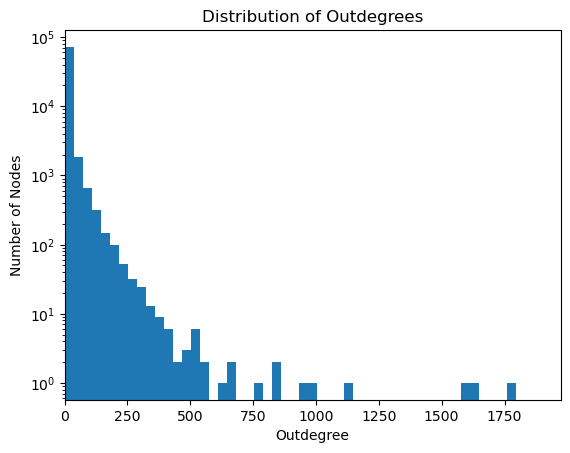
\includegraphics[width=0.4\textwidth]{epinions_outdegree_distr}
    \caption{Distribution of outdegrees in the Epinions graph.}
    \label{fig:epinions_outdegrees}
\end{figure}

Before discussing the runtime of the power resolution, we will first explore relevant and interesting statistics that the resolving revealed. 330 closed delegation cycles were collapsed, which affected 740 nodes, about 0.01\% of nodes in the graph. This means each closed delegation cycle has an average length of 2.24 nodes. The most powerful node after resolving is the "lost" node, so the node where power goes, that was delegated into closed delegation cycles. This node's power, together with the power of the 740 nodes that were removed before removing due to being inside of a closed delegation cycle, adds up to 2777.056087, which accounts for about 0.037\% of power in the graph. The distribution of powers after resolving is shown in \cref{fig:epinions_powers}.

\begin{figure}[h]
    \centering
    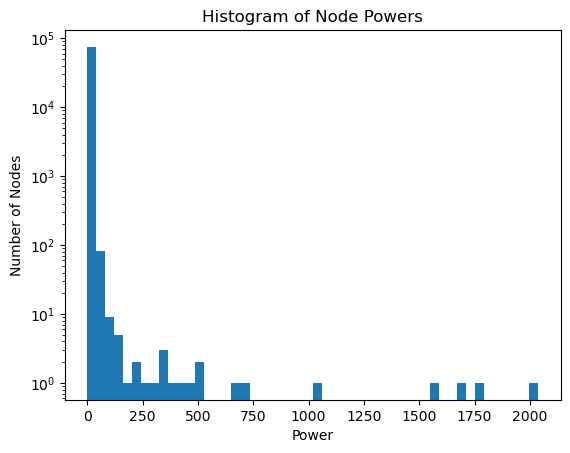
\includegraphics[width=0.4\textwidth]{epinions_power_distr}
    \caption{Distribution of node powers in the Epinions graph.}
    \label{fig:epinions_powers}
\end{figure}

The runtimes of each implementation to resolve the Epinions Graph's runtime are shown in \cref{fig:epinions_runtimes}. 

\begin{figure}[h]
    \centering
    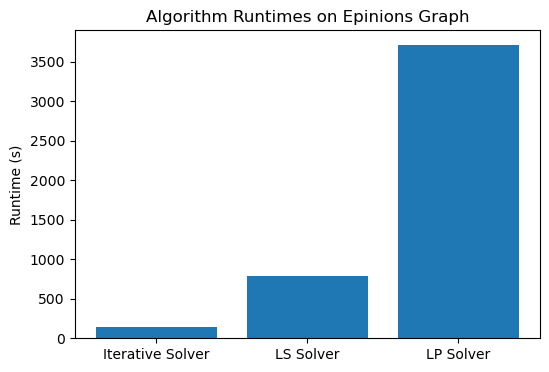
\includegraphics[width=0.4\textwidth]{epinions_dataset}
    \caption{Runtime of delegation algorithms on the Epinions Graph.}
    \label{fig:epinions_runtimes}
\end{figure}

\TODO{ADD THE ACTUAL EVALUTION. I WANT TO FIRST DISPLAY THE RESULTS OF THE OTHER TWO METHODS AS WELL, SO THAT I DON'T END UP REPEATING MYSELF TOO OFTEN. MAYBE THE EVALUATION CAN BE BUNDLED FOR ALL THREE METHODS...}

\TODO{Fix and make more clean the captions for runtime graphs. Currently they mention "delegation algorithms", which is outdated terminology}

\subsection{Bitcoin OTC Trust Network}

Users trading Bitcoin on the platform "Bitcoin OTC" maintain a record of trust to other users, in order to prevent transactions with untrustworthy users. SNAP provides the Bitcoin OTC Trust Graph, a graph of this trust between users. \TODO{cite: \url{https://snap.stanford.edu/data/soc-sign-bitcoin-otc.html}} The graph is directed and weighted, with weights ranging from -10 to 10, total distrust to total trust. \TODO{cite: \url{https://snap.stanford.edu/data/soc-sign-bitcoin-otc.html}} 

The graph was first cleaned, to remove all edges with a non-positive trust values, before being turned into a well-formed delegation graph as per fig XX, again not adding any sinks artificially. The preprocessing pipeline normalizes edge weights, meaning outgoing trust levels are scaled down proportionally to add up to one, preserving relative differences in trust. The finished graph contains 5573 nodes, of which 806 are sinks, about 0.15\%. The outdegree distribution in the Bitcoin OTC Trust Graph are shown in \cref{bitcoinotc_outdegrees}.

\begin{figure}[h]
    \centering
    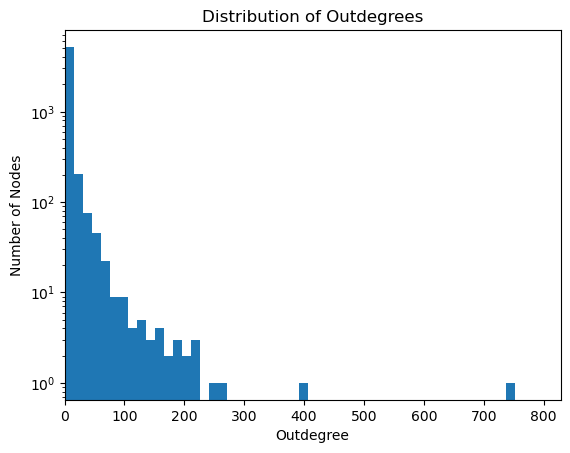
\includegraphics[width=0.4\textwidth]{bitcoinotc_outdegree_distr}
    \caption{Distribution of outdegrees in the Bitcoin OTC Trust Graph.}
    \label{fig:bitcoinotc_outdegrees}
\end{figure}

During the preprocessing of this graph, 43 of the graph's 5573 nodes were to be removed since they were in a closed delegation cycle, yielding an average length of closed delegation cycles of about 2,38. In total, in this graph, about 111.2 units of power were lost to closed delegation cycles, about 0.02\% of the total power in the graph. The distribution of powers after resolving is shown in \cref{fig:bitcoinotc_powers}

 \begin{figure}[h]
    \centering
    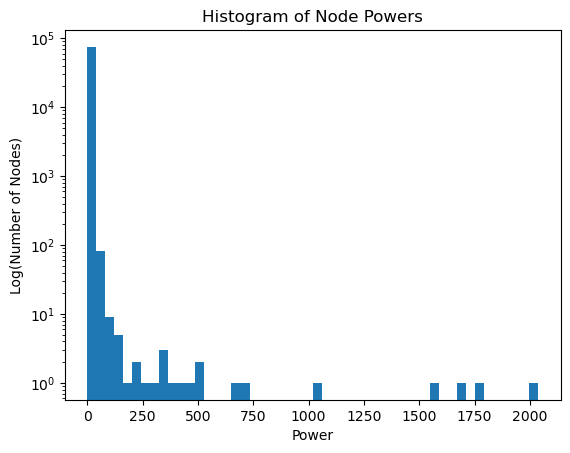
\includegraphics[width=0.4\textwidth]{bitcoinotc_power_distr}
    \caption{Distribution of powers in the Bitcoin OTC Trust Graph.}
    \label{fig:bitcoinotc_powers}
\end{figure}

\begin{figure}[h]
    \centering
    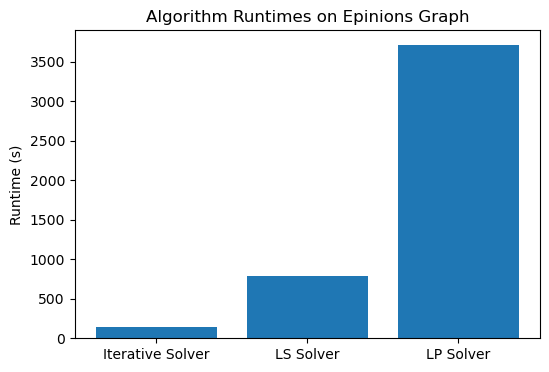
\includegraphics[width=0.4\textwidth]{bitcoinotc_dataset}
    \caption{Runtime of delegation algorithms on the Bitcoin OTC Trust Graph.}
    \label{fig:bitcoinotc_runtimes}
\end{figure}
 
\TODO{Same here, still do the evaluation}

\subsection{Slashdot Zoo}

The Slashdot technology news size provides a so-called "zoo" feature, in which users can tag other users as friends and foes. \TODO{Cite: \url{https://dai-labor.de/en/publications/the-slashdot-zoo-mining-a-social-network-with-negative-edges/}}
 The Distributed AI Laboratory in Berlin (DAI Labor) provides a graph based on this data. \TODO{Cite: \url{https://dai-labor.de/en/publications/the-slashdot-zoo-mining-a-social-network-with-negative-edges/}} It is a directed and weighted graph, where an edge weight of +1 indicates a friend relationship, and an edge weight of -1 indicates a foe relationship.
 
 \begin{figure}[h]
    \centering
    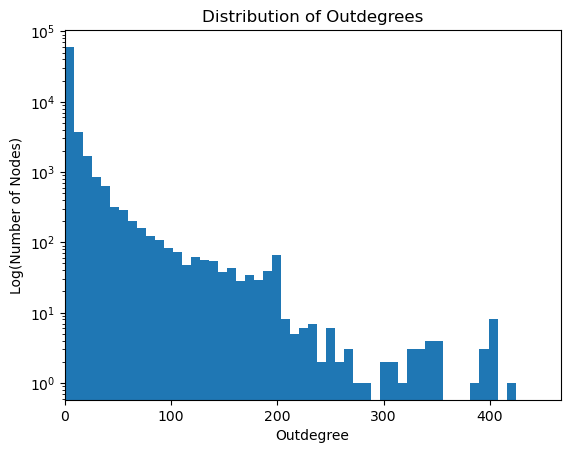
\includegraphics[width=0.4\textwidth]{slashdot_outdegree_distr}
    \caption{Distribution of outdegrees in the Slashdot Zoo Graph.}
    \label{fig:slashdot_outdegrees}
\end{figure}


 \begin{figure}[h]
    \centering
    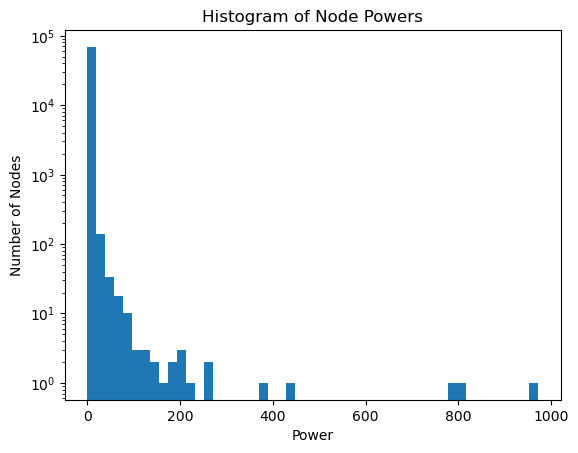
\includegraphics[width=0.4\textwidth]{slashdot_power_distr}
    \caption{Distribution of powers in the Slashdot Zoo Graph.}
    \label{fig:slashdot_powers}
\end{figure}

 \begin{figure}[h]
    \centering
    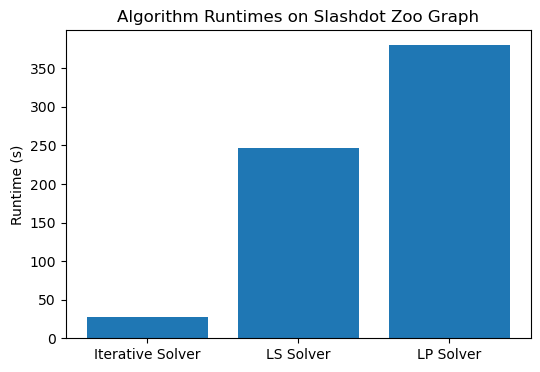
\includegraphics[width=0.4\textwidth]{slashdot_dataset}
    \caption{Runtime of delegation algorithms on the Slashdot Graph.}
    \label{fig:slashdot_runtimes}
\end{figure}




\TODO{Maybe mention also at some point, that this evaluation is a comparison between different solvers for systems of linear equations}

\TODO{Mention that the iterative solver is a lot less precise}